\documentclass[../main.tex]{subfiles}
\begin{document}

% Allgemeines Kapitel "Sicherheitsuntersuchungen" mit Intro a la:

% Lange Liste an Empfehlungen/best practices für Docker:
%		- einige einfache, die automatisch von Docker erzwungen werden
%		- einige nicht offensichtliche, die manuell aktiviert werden müssen
%		- einige schwierige, die keine Kernel-Unterstützung haben
%	^		\cite[S.10]{presContainerDockerSec}

% Kleinere Angriffsoberfläche für Container durch minimal distros (alpine linux, buildroot, atomic?)
%		- Und durch Tatsache, dass HW-Management komplett auf dem Host gemacht wird, nicht in den Containern
%	^		\cite[S.16]{presContainerDockerSec}

% Immutable Containers mit "docker run --read-only"
%	^		\cite[S.17]{presContainerDockerSec}

% Image Trusting: Imageersteller, Operator der Registry, Transport zwischen Client und Hub
%	^		\cite[S.18]{presContainerDockerSec}

% Security kommt oft mit Usability-Einbußen (was mit Ease of Use eine Stärke von Docker ist)
%	^		\cite[S.26]{presContainerDockerSec}

% Docker Security Zukunft>
%	- noexec, nosuid für immutable containers
%	- bessere GRSEC, PAX, LSM integration
%	- user namespaces
%	- bessere default seccomp profiles
%	^		\cite[S.40]{presContainerDockerSec}

% Zitat vllt mit in eine DockerSecurity Einleitung:
% "A year ago, Docker and security was pretty horrible, six months ago it wasn't so bad, and now it's pretty usable."
% von David Mortman at DEFCON (WELCHES JAHR IST NOCH WICHTIG)
% a la.. "wir untersuchen was er meint, was sich verbessert hat etc."
%	^		\cite[S.41]{presContainerDockerSec}

% Angreifer können ein paar Angriffe ausführen: Privilege escalation und Denial of Service.
%  °	\cite[S.3]{dockerSec1}

\chapter{Security aus Linux Kernel-Features}
\label{secLinux}
  % namespaces/etc (was es ist) in Einleitung mit rein? 1.) Erklaeren, 2.) Security/Docker untersuchen dazu im Security Hauptteil
  % 2 Unterkapitel, inhatliche Überschneidung evtl., Grund nennen warum so gegliedert, ...
  % \cite[S.3]{dockerIntroIEEE} --> umgangsprachlich erkleart wie mit namespaces und cgroups gearbeitet wird

	% User namespaces are only one piece of the puzzle. AppArmor/SELinux, Notary, image security, and proper environment/network security all play a part in the overall Docker security picture
	%  ^ 	\cite[S.7]{nsUserContainerCon}

	\section{Isolierung durch \texttt{namespaces}}
  \label{secIsolierung}
		Wenn unter Linux ein neuer Prozess gestartet werden soll, wird über \emph{System Calls} dem Kernel mitgeteilt, einen neuen \emph{namespace} bereitzustellen. Je nach Anforderung gibt es verschiedene \emph{namespaces}, z.B. ein \emph{network namespace}, der dem neuen Prozess ein Netzwerkinterface zuweist. Um Container als isolierte Arbeitsbereiche auf einem Host zu erstellen, werden die \emph{namespaces} des Kernels verwendet. Da Container selbst eine eigene komplette Laufzeitumgebung darstellen sollen, müssen Bereiche des Hosts durch \emph{namespaces} abgedeckt sein, sodass neben dem Netzwerk auch z.B. ein beschränkter Zugriff auf den Arbeitsspeicher und die \acrshort{CPU} gewährleistet ist \cite[S.3]{dockerIntroIEEE}.

		Technisch betrachtet beinhaltet ein \emph{namespace} eine Lookup-Tabelle, die global verfügbare Ressourcen abstrahiert und dem \emph{namespace} bereitstellt. Änderungen globaler Ressourcen sind sichtbar für Prozesse im relevanten \emph{namespace}, jedoch unsichtbar für solche außerhalb \cite[S.1+2]{IBMcheckpointRestart}\cite{namespaces}. Dadurch können \emph{namespaces} als Lösungsansatz des Sicherheitsziels Vertraulichkeit betrachtet werden. Sie sind damit der wesentliche Baustein, um eine Containerisolierung zu realisieren.
		% Nach ..(reshetova).. müssen Anforderungen an Prozessisolierung, Dateisystemisolierung, Geräteisolierung, Prozessisolierung und Netzwerklimitierung erfüllt sein.

    % Isolierung erklären, erfüllt X Schutzziele, Bezug auf Forschungsfrage
    % Es gibt 6 Namespaces, die im folgenden *anhand der verschiedenen Betriebssystemkomponenten?) untersucht werden.

		% Unfortunately, the namespace support code is complicated and in the past, various bugs have allowed applications to escape from this namespace isolation and interfere with other containers. The known bugs have been fixed.
		%		^		\cite{ https://coreos.com/blog/container-security-selinux-coreos.html }

		\subsection{Prozessisolierung durch den \texttt{\acrshort{PID} namespace}}
		\label{secIsoProcesses}

			Jeder Container entspricht auf dem Host zunächst einem Prozess. Da die Container untereinander isoliert sein sollen, dürfen auch die zugrundeliegenden Containerprozesse nicht miteinander interferieren.

			Docker erreicht diese Isolierung auf Prozessebene durch die Nutzung des \emph{\acrshort{PID} namespace}, in denen Container eingebettet werden. Nach diesem hierarchischen Konzept ist es einem Prozess X nur möglich, selbsterzeugte Kindprozesse zu beobachten und mit ihnen zu interagieren. Elternprozesse, also Prozesse die in der Prozesshierarchie über X stehen, sind für X unsichtbar. Der Elternprozesse haben jedoch die volle Kontrolle über X und können diesen z.B. jederzeit mit dem Befehl \texttt{kill} beenden. Darüber hinaus haben Elternprozesse die Möglichkeit mit z.B. einem Aufruf von \texttt{ps} alle Kindprozesse überwachen.

			Übertragen auf die containerbasierte Virtualisierung bedeutet das, dass der Host vollen Zugriff auf die laufenden Container hat, Containerprozesse jedoch weder Kenntnis von Hostprozessen noch von Prozessen anderer Container besitzen (vgl. \fig \ref{fig:sec_pidNsHost} und \fig \ref{fig:sec_pidNsContainer}). Diese Eigenschaft macht es Angreifern schwieriger Schaden anzurichten, da sie ausgehend von kompromitierten Containern keine Informationen über Prozesse außerhalb des Containers beziehen können.

			Ein weiterer Mechanismus des \emph{\acrshort{PID}-namespace} ist eine Besonderheit des Prozesses mit \texttt{PID=1}. Der initiale Containerprozess kann mit der \texttt{PID=1} gestartet werden, dem es als \emph{init}-ähnlicher Prozess möglich ist, alle Kindprozese zu terminieren sobald er selbst beendet wird. Somit können komplette Container durch einen Hostzugriff auf den Containerprozess mit \texttt{PID=1} umgehend vollständig heruntergefahren werden.

			Wie sich der \emph{\acrshort{PID}-namespace} auf einen gestarteten Docker-Container auswirkt, ist in \fig \ref{fig:sec_pidNsHost} und \fig \ref{fig:sec_pidNsContainer} zu sehen.

			\begin{figure}[h]
					\centering
					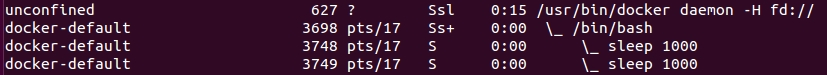
\includegraphics[width=1.0\textwidth]{./images/sec_pidNsHost.jpg}
					\caption{Ausschnitt der Ausgabe des Befehls \texttt{ps -eaxfZ} auf einem Docker-Host (eigene Abbildung).}
					\label{fig:sec_pidNsHost}
			\end{figure}

			\fig \ref{fig:sec_pidNsHost} stellt einen Auschnitt der Ausgabe des Befehls \texttt{ps -eaxfZ} auf dem Host dar. Er enthält die laufenden Docker-Prozesse des Daemons mit \texttt{PID=627} (Zeile 1) und einem Container, in dem eine \emph{Bash} gestartet wurde (Zeile 2). Innerhalb der \emph{Bash} wurde der Befehl \texttt{sleep 1000} zweifach ausgeführt (Zeile 3 und 4), der laufende Hostprozesse zurückgibt. Wie zu erkennen ist, sind die Containerprozesse aus Sicht des Hosts mit einer eigenen \texttt{PID} vollkommen transparent.

			\begin{figure}[h]
					\centering
					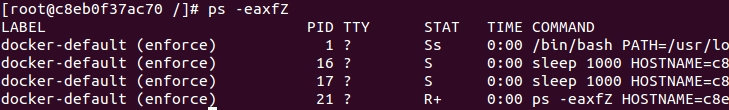
\includegraphics[width=1.0\textwidth]{./images/sec_pidNsContainer.jpg}
					\caption{Ausgabe des Befehls \texttt{ps -eaxfZ} in einem Docker-Container (eigene Abbildung).}
					\label{fig:sec_pidNsContainer}
			\end{figure}

			\fig \ref{fig:sec_pidNsContainer} zeigt die vollständige Ausgabe des gleichen Befehls innerhalb eines Containers. Prozesse außerhalb des Containers sind unsichtbar. Außerdem weisen die Containerprozesse im Vergleich zu \fig \ref{fig:sec_pidNsHost} nun eine andere \texttt{PID} auf. Da die \emph{Bash} der initiale Containerprozess ist, erhält sie die \texttt{PID=1}.

			%Fast alles bisher:


			% PID namespaces sind hierarchisch http://lwn.net/Articles/259217/

			% Einzelnen Containerlösungen unterscheiden sich nur geringfügig. Alle nutyen namespace, cgroups, chroot.
			% Unterschiede im Contaier lifecycle jedoch (docker sehr gut aufgestellt --> teil von dockers erfolg beruht darauf)
			%	^		\cite[S.4]{virtVSContainer}

			% TODO: init-ähnlicher Prozess im Glossar erklären
			% TODO: Grafik mit Prozess PIDs und Hierarchie einbinden

    \subsection{Dateisystemisolierung durch den \texttt{mount namespace}}
			Auch das Hostdateisystem muss von unrechtmäßigen Zugriffen aus Containern geschützt werden.

			Dateisysteme sind allgemein wie Prozesse in Kapitel \ref{secIsoProcesses} hierarchisch aufgebaut. Diese können mithilfe von \emph{mount namespace} unterteilt werden, sodass unter Docker jeder Container eine andere Sicht auf die Verzeichnisstruktur des Hosts hat. Nur ein bestimmtes Unterverzeichnis ist für einen Container sichtbar, wenn er dieses als Mountpoint einbindet.

			Eine Hostverzeichnisse werden jedoch nicht in den \emph{mount namespace} eingezogen, weil sie von den Docker-Containern benötigt werden, um zu operieren.

			Dazu gehören die Verzeichnisse:

			\begin{itemize}
				\item \texttt{/sys}:
				\item \texttt{/proc/sys}:
				\item \texttt{/proc/sysrq - trigger}:
				\item \texttt{/proc/irq}:
				\item \texttt{/proc/bus}:
			\end{itemize}

			Als Konsequenz erben Container diese notwendigen Verzeichnisse direkt von ihrem Host, was ein Sicherheitsrisiko darstellt. Docker dämmt dieses ein, indem es nur einen reinen Lesezugriff ohne Schreibrechte auf diese Verzeichnisse erlaubt \cite[S.4]{dockerSecIntro}. Außerdem ist es Containern unter Docker nicht erlaubt, Hostverzeichnisse erneut einzubinden, um Schreibrechte sicher auszuschließen. Dieses Verbot wird durch die Verweigerung der \emph{capability} bla \texttt{CAP\_SYS\_ADMIN} für Container erreicht.
			% TODO: Einbinden: Dateisysteme werden gemountet unter der Angabe der Berechtigung, also ob read oder write. EIn remount ist daher gefährlich.

			Durch das von Docker genutzte und bereits in Kapitel \ref{dockerImages} beschriebene \emph{\acrshort{COW}}-basierte Dateisystem, ist es jedem Container möglich, Änderungen in seinem durch den \emph{mount namespace} zugewiesenen Verzeichnis zu speichern. Containerdaten interferieren dadurch nicht und sind containerübergreifend nicht sichtbar, auch beim Betrieb von Containern, die auf einem gleichen Basisimage beruhen \cite[S.4]{dockerSecIntro}.

			% Dieser namespace basiert auf chroot()
			%	^		\cite[S.3]{virtVSContainer}

			%Fast alles bisher:
			\cite[S.4]{dockerSec1}

			% Filesystem Isolation kann mit user namespaces verstaekrt werden, indem user und groups IDs auf wenige rpriveliigierte host uids und group ids gemappt werden. Zusammen mit dem mount namespace und einer pivot_root umgebung kann das den schutz fuer filesystembasierte Attacken erhoehen
			%		^ 	\cite[S.11]{dockerSec2}

    \subsection{Geräteisolierung durch ....}
			% Es gibt keinen richtigen Namespace dafuer, da linux device driver (die physischen devices kontrollieren), nicht namespace aware sind und damit nicht sicher in containern verwendet werden koennen
			% Nur die Cells-Implementierung baut einen 'device namespace'
			% Sonst nur ueber capabilities einschraenkbar (gennant im text: CAP_SYS_MKNOD)
			%		^ 	\cite[S.12]{dockerSec2}

			In Unix-basierenden Betriebssystemen wie Linux erfolgt der Zugriff auf Hardware über sogenannte \emph{Device Nodes}, die in dem Dateisystem von speziellen Dateien repräsentiert sind.
			% TODO: Device Nodes ins Glossar aufnehmen. Dort dann sagen, dass es speyielle Files sind etc.

			Ein paar wichtige \emph{Device Nodes} und deren Zuständigkeiten sind im Folgenden aufgeführt.

			\begin{itemize}
				\item \texttt{/dev/mem}: Arbeitsspeicher
				\item \texttt{/dev/sd*}: Files für den Zugriff auf Speichermedien
				\item \texttt{/dev/tty}: Terminal
			\end{itemize}

			Wie zu sehen ist, handelt sich dabei um teils äußerst kritische Komponenten einer Maschine, über die Container unter keinen Umständen verfügen dürfen. Deswegen ist es notwendig den Zugriff auf \emph{Device Nodes} stark einzuschränken, um den Host vor Missbrauch zu schützen.
			% TODO: Starke Abhängigkeit zu cgroups (guten Übergang machen bzw. Abgrenzung)

			% Standardmaessig haben Container keinen zugriff auf Devices. Kann aber explizit bei container launch anders festgelegt werden \cite[S.4]{dockerSecIntro}

			%Fast alles bisher:
			\cite[S.4]{dockerSec1}

			% Problem mit PseudoRandomNumberGenerator in /dev/random und /dev/urandom, da das blocking devices sind
			%		^ 	\cite[S.18]{dockerSec2}

			% Problem mit HotPlug Support unter Linux
			%		^ 	\cite[S.19]{dockerSec2}

    \subsection{\acrshort{IPC}-Isolierung durch den \texttt{\acrshort{IPC}-namespace}}
			Unter \acrshort{IPC} versteht man ein Sammlung an Tools, die für den Datenaustausch zwischen Prozessen genutzt werden. Dazu gehören z.B. \emph{Semaphoren}, \emph{Message Queues} und \emph{Shared Memory Segments}.

			Ergänzend zu dem \emph{\acrshort{PID} namespace}, der die Sichtbarkeit sowie Kontrolle über Prozesse in der Prozesshierarchie einschränkt, kann auch die Kommunikation zwischen Prozessen limitiert werden.

			Docker gewährleistet dies durch den Zuweisung eines \emph{\acrshort{IPC}-namespaces} pro Container, in dem ein Prozesse nur mit anderen Prozessen in Kontakt treten kann, wenn sich diese in einem gleichen \emph{\acrshort{IPC}-namespace} befinden. Eine versehentliche oder beabsichtige Interferenz mit Prozessen des Hosts oder anderer Container wird damit ausgeschlossen.

			%Fast alles bisher:
			\cite[S.4]{dockerSec1}

			% Problem mit TIPC Extension, wo ipc namespace umgangen werden kann
			%		^ 	\cite[S.18]{dockerSec2}

    \subsection{\acrshort{UTS}-Isolierung durch den \texttt{\acrshort{UTS}-namespace}}
			\emph{Nur der Vollständigkeit halber aufgelistet? Oder hat der Relevanz für Container?}
			\emph{weniger sicherheitsrelevant oder...}
			Mit einem \emph{\acrshort{UTS}-namespace} ist es möglich jedem Container einen eigenen Hostnamen zuzuweisen. Der Container kann diesen Namen abfragen und ändern \cite[S.3]{virtVSContainer}.
    \subsection{Netzwerkisolierung durch den \texttt{network namespace}}
			Um einen sicheren Betrieb von Docker zu gewährleisten, müssen Container so konfiguriert sein, dass sie weder den Netzwerkverkehr des Hosts noch anderer Container abhören oder manipulieren können.

			Dazu stellt Docker jedem Container einen eigenen unabhängigen Netzwerk-Stack zur Verfügung, der durch \emph{network namespaces} realisiert wird. Jeder Namespace hat seine eigene private IP-Adresse, IP-Routingtabelle, Loopback-Interface und Netzwerkgeräte \cite[S.2+3]{virtVSContainer}. Eine Kommunikation zu anderen Containern auf dem gleichen oder entfernten Hosts geschieht dann über diese dafür vorgesehenen Schnittstellen.

			Um die oben genannten Netzwerkressourcen anzubieten, wird jedem \emph{network namespace} ein eigenes \texttt{/proc/net}-Verzeichnis zugewiesen. Die Nutzung von Befehlen wie \texttt{netstat} und \texttt{ifconfig} wird damit, aus einem \emph{network namespace} heraus, auch ermöglicht \cite[S.7]{IBMcheckpointRestart}.

			Standardmäßig wird von Containern eine \emph{Virtual Ethernet Bridge} namens \texttt{docker0} genutzt, um mit dem Host oder anderen Containern zu kommunizieren. Neu gestartete Container werden dieser Bridge hinzugefügt, indem deren Netzwerkinterface \texttt{eth0} mit der Bridge verbunden wird. Aus Sicht des Hosts ist das Interface \texttt{eth0} ein virtuelles \texttt{veth}-Interface \cite[S.3]{virtVSContainer}.

			Die Bridge leitet ohne Filter alle eingehenden Pakete weiter, welchen Umstand dieses Verbindungsdesign anfällig gegenüber \acrshort{ARP}-Spoofing und \acrshort{MAC2}-Flooding macht. Diesem Nachteil kann Abhilfe geschafft werden, indem manuelle Filtermethoden mittels beispielsweise \emph{ebtables} in die Bridge integriert werden, oder ein anderes Verbindungsdesign auf basis virtueller Netzwerke gewählt wird.
			% TODO: Im Glossar die beiden Angriffe erklären?
			% TODO: ebtables besser erklaeren falls noch relevant http://ebtables.netfilter.org/

			% TODO: Bild zu Bridge-Layout (z.B. in dockerSec1, s.5, oben)

			% TODO: Integrieren: https://docs.docker.com/engine/userguide/networking/

			%Fast alles bisher:
			\cite[S.4]{dockerSec1}

			% network namespace:
	    % Standardmäßig werden für Container keine Ports geöffnet. Manche Applikationen machen jedoch nur Sinn, wenn sie Ports nutzen können, daher können diese manuell in dem Dockerfile (INTERNE REFERENZ) freigegeben werden.
	    % Container werden virtuelle Netzwerkinterfaces zur Verfügung gestellt. Dadurch können z.B. mehrere Container betrieben werden, die Webserver beinhalten, die alle auf Port 80 eingestellt sind. Außerhalb der Container können diese Containerports mithilfe von NAT (sicher NAT?) auf unterschiedliche Ports des Hosts abgebildet werden.
	    %  ^ \cite[S.3]{dockerIntroIEEE}

    \subsection{Userisolierung (user namespace)}
			Bislang werden Container unter Docker und anderen linuxbasierten Containerlösungen mit Root-Rechten gestartet. Falls es einem Angreifer in diesem Szenario gelingt, aus der Containerisolation auszubrechen, ist er automatisch Root-User auf dem Host, was ein hohes Sicherheitsrisiko ist. Durch die potentielle Gefahr dieser Vorgehensweise, wird die Einführung von \emph{user namespaces} als Meilenstein der Containersicherheit gewertet.
			% TODO: Quelle hinzufuegen .. blog artiekl etc.
			% schlechte Quelle...: http://rhelblog.redhat.com/2015/07/07/whats-next-for-containers-user-namespaces/
			% Root-Rechte wurden bisher mit capabilities eingeschränkt.

			Dieser Kernel-\emph{namespace} führt einen Mechanismus ein, unter dem Rootrechte in Containern nicht Rootrechten auf dem Host entsprechen, in anderen Worten ein Root-User im Container auf einen Nicht-Root-User auf dem Host aufgelöst wird. Durch das potentielle Sicherheitsrisiko der bisherigen Vorgehensweise,

			Linux verwendet \emph{User IDs} (\texttt{uids}) und \emph{Group IDs} (\texttt{gids}), um Verzeichnisse und Dateien eines Dateisystems sowie Prozesse mit Eignerinformationen zu versehen. \emph{user namespaces} erlauben unterschiedliche \texttt{uids} und \texttt{gids} innerhalb und außerhalb des \emph{namespace}. Im Kontext des Hosts kann dadurch ein unpriveligierter User (ohne Root-Rechte) existieren, während der gleiche User innerhalb von Containern mit \emph{user namespace} priveligiert ist, also im Besitz von Root-Rechten ist \cite{nsUser}.

			In der Praxis lasen sich mit diesem Konzept jeweils Root-User mit \texttt{uid=0} in Container X und Y auf nicht-priviligierte User mit \texttt{uid=1000} und \texttt{uid=2000} des Hosts abbilden.
			% TODO: Grafik zur Unterstuetzung waere gut hier...


			Die Unterstützung von \emph{user namespaces} ist schon seit Version 1.6 geplant, wurde aber erst im Februar 2016 mit Version 1.10 in den Master-Branch von Docker integriert \cite{githubDockerChangelog}\cite{githubUserNamespaceProposal}. Verzögerungen entstanden durch einen Bug der Programmiersprache \emph{Golang} \cite{nsUserGolangBug}, und Integrationschwierigkeiten in die bestehende Docker-Codebasis \cite{githubUserNamespaceConflict}.

			In der aktuell neusten Docker-Version 1.10 werden \emph{user namespaces} nicht automatisch verwendet. Sie müssen manuell, wie z.B. in \cite{nsUserEnable} erklärt, aktiviert werden.

			% Mehr (Bessere) Gruende: http://events.linuxfoundation.org/sites/events/files/slides/User%20Namespaces%20-%20ContainerCon%202015%20-%2016-9-final_0.pdf
			% S.13ff.

			Beide Probleme sind jedoch mittlerweise gelöst, wie die erfolgreiche Integration von \emph{user namespaces} in Docker im Oktober 2015 bestätigt \cite{githubUserNamespaceIntegration}. Dadurch, dass \emph{user namespaces} in der Docker-Roadmap als wichtiges Sicherheitsfeature gesehen werden, ist ein Release dessen bald zu erwarten \cite{githubDockerRoadmap}.

			% A single-threaded process can join another user namespace with setns(2) if it has the CAP_SYS_ADMIN in that namespace; upon doing so, it gains a full set of capabilities in that namespace.
			%		^ 	\cite{nsUser}

      % \texttt{user namespaces} ist Future implementation, da neues Kernelfeature. Trotzdem Konzept erklären und wie Docker-Security davon profitiert.

			% User namespace is the only namespace which can be created without CAP_SYS_ADMIN capability
			% aus: http://www.haifux.org/lectures/299/netLec7.pdf .... Seite 61

			Auch für Cloudanbieter sind \emph{user namespaces} von Vorteil: Mit einer Auflösung der Container auf Userebene ist es einerseits möglich Servicenutzung auf Userbasis einzugrenzen und andererseits diese auf Userbasis abzurechnen. Wenn ohne \emph{user namespaces} jede gestartete Containerinstanz einem Hostuser mit \texttt{uid=0} zugehörig ist, gestaltet sich die Zuordnung schwieriger \cite[S.3]{nsUserContainerCon}.
	\section{Ressourcenverwaltung / Limitierung von Ressourcen durch \texttt{\acrshort{cgroups}}}
  \label{secResLimit}
		\acrshort{DoS}-Attacken mit der Absicht das Sicherheitsziel der Verfügbarkeit zu verletzen, gehören in \gls{MultiTenantService}-Systemen zu einem gängigen Angriffsmuster \cite[S.5]{dockerSec1}. Um die Verfügbarkeit von Containern sicherzustellen, bietet der Linux-Kernel sogenannte \emph{\acrlong{cgroups}} (kurz \texttt{\acrshort{cgroups}}) an, die auch von Docker genutzte Möglichkeiten zum Ressourcenmanagement bereitstellen.


		% \emph{control groups}, oder auch verkürzt \emph{cgroups} genannt, ist hierbei das Schlüsselfeature des Linuxkernels, um dieser Art von Angriff entgegenzuwirken. Sie stellen sicher, dass jeder Container nur begrenzt Hostressourcen beansprucht. Mit Docker lassen sich Limits und Bedingungen individuell pro Container anpassen, z.B. an einen bestimmten Container gerichtetes Arbeitsspeicherlimit in Bytes, das ihm maximal im Betrieb zur Verfügung steht \cite[S.4]{dockerSecIntro}.
		% --> Quelle aus docker docs findbar?

		\texttt{\acrshort{cgroups}} sind historisch aus dem Konzept von sogenannten \emph{\acrlong{rlimits}}, auch \texttt{\acrshort{rlimits}} genannt, gewachsen. Mit \emph{rlimits} werden \gls{weicheHarteLimits} definiert, die pro Prozess angewandt werden. Der Betrieb von Contaiern verlangen jedoch eine Ressourcenverteilung auf Containerbasis, sodass Limits pro Container, aus technischer Sicht einem Set an Prozessen, vergeben werden.
		% TODO: rlimits abgleichen mit \cite[fundamentalkapitel]{linuxInterface}

		%Dieses minimale Konzept auf Prozessebene ist für den Betrieb moderner Container jedoch unzureichend, da u.a. keine Beschränkungen auf Containerebene, also für Prozessgruppen, vorgenommen werden können. % z.B. keine Aktionen festgelegt werden können, die ausgeführt werden, wenn ein solches Limit erreicht ist. Außerdem können die \acrshort{CPU} und der Speicher nur begrenzt von \emph{\acrlong{rlimits}} kontrolliert werden.

		Viele Containertechnologien erweiterten deswegen \texttt{\acrshort{rlimits}} mit eigenen Features. Z.b. fügten die Entwickler von \emph{FreeBSD} für den Betrieb von \emph{Jails} sogenannte \emph{Hierarchical Resource Limits} hinzu \cite{freeBsdRCTL}. \emph{Solaris} bietet die Nutzung von \emph{Resource Pools} an, die eine Partitionierung von Ressourcen implementiert \cite{cgroupsUniHierarchyDoc}. Auch \emph{OpenVZ} und \emph{Linux-VServer} erweitern \texttt{\acrshort{rlimits}}, sodass Ressourcenlimits pro Container definiert werden können \cite[S.15+16]{dockerSec2}.

		Die Nachteile von \texttt{\acrshort{rlimits}} wurden mit der Implementierung von \texttt{\acrshort{cgroups}} für den Linux-Kernel behoben. Mit diesem relativ neuen Mechanismus werden Prozesse in hierarchischen Gruppen angeordnet, die individuell verwaltet werden und deren Attribute vererbt werden können. Neben vielseitiger und feingranularer Funktionen zum Management von z.B. \acrshort{CPU}- und Speicherressourcen, können unter \texttt{\acrshort{cgroups}} komplexe Verfahren implementiert werden, die zur Korrektur von limitüberschreitender Prozesse dienen \cite{cgroupsRedhat}. Die Implementierung von \texttt{\acrshort{cgroups}} wurde ab 2012 weiter verbessert, sodass eine Update unter dem Namen \emph{Unified Control Group Hierarchy} seit 2014 in den Linux-Kernel integriert ist \cite{cgroupsFixing}\cite{cgroupsUniHierarchy}. Von Docker wird die neue \emph{Unified Hierarchy} noch nicht verwendet \cite{ https://github.com/docker/docker/issues/16238 }

		Wichtig zu erwähnen ist, dass die Implementierung von \texttt{\acrshort{cgroups}} verglichen mit der von \texttt{\acrshort{rlimits}} angeblich noch nicht vollständig ist. Das Feature Dateisysteme als Ressourcen mit \texttt{\acrshort{cgroups}} zu steuern, fehlt nach Angaben von \cite[S.19]{dockerSec2}. Auch im Quellcode von \emph{runC} ist eine Dateisystem-Interface als \glqq{}nicht unterstützt\grqq{} gekennzeichnet und wird demzufolge auch nicht von Docker genutzt. \cite{githubRunCCgroups}. Diskussionen im \emph{GitHub}-Repository von Docker verweisen in Bezug zu diesem Feature auf Abhängigkeiten zur Art des Dateisystems. Offenbar lassen sich sogenannte Dateisystem-Quotas nur mit \emph{Device Mapper} und \emph{Brtfs} softwaretechnisch lösen, \emph{AuFS} jedoch ermöglicht das nur indirekt über die Zuweisung von Festplattenpartitionen fester Größe. Diese Gegebenheit lässt vermuten, dass eine universelle Lösung aktuell an der Breite unterstützter Dateisysteme scheitert \cite{githubDockerIssueFsQuota}. Die neusten Entwicklungen sehen jedoch eine Quota-Implementierung vor \cite{githubDockerPullBrtfs}.

		Dennoch ist diese Erweiterung im Sinne einer einheitlichen Verwaltung von Ressourcen mit \texttt{\acrshort{cgroups}} vorgesehen \cite[S.16+19]{dockerSec2}.

		Alle gängigen Linux-basierten Containerlösungen, darunter auch Docker, nutzen aktuell \texttt{\acrshort{cgroups}}, um Ressourcen für Container zu verwalten \cite[S.16]{dockerSec2}. Der Einsatz von \texttt{\acrshort{cgroups}} unter Docker umfasst, wie im Quellcode von \emph{runC} zu sehen ist, die Kontrolle über \acrshort{CPU}, Arbeitsspeicher, Geräte (\emph{Devices Nodes}, Netzwerkinterfaces und \acrshort{I/O}-Operationen auf Speichermedien wie \acrshort{HDD}, \acrshort{SSD} und \acrshort{USB}-Speicher \cite{cgroupsRedhat}\cite{githubRunCCgroups}.

		Über die Kommandozeile lässt sich der \texttt{run}-Befehl, der ausgeführt wird, um einen Container zu starten, mit Angaben zur Ressourcennutzung parametrisieren. Z.b. bewirkt die Hintereinanderausführung folgender Befehle, dass dem zuletzt gestarteten Container doppelt so viel CPU-Leistung zur Verfügung gestellt wird, wie dem ersten Container \cite{dockerRun}.

		\begin{lstlisting}
			user@machine:$ docker run <IMAGE> --cpu-shares=50
			user@machine:$ docker run <IMAGE> --cpu-shares=100
		\end{lstlisting}

		Neben dem Ressourcenmanagement bieten \texttt{\acrshort{cgroups}} auch Nutzungsstatistiken an. Diese können unter Docker mit dem Befehl \texttt{docker stats <CONTAINER> [<CONTAINER>]} abgerufen werden \cite{dockerMetrics}.

		% TODO: Evtl. stress test aus
		% https://goldmann.pl/blog/2014/09/11/resource-management-in-docker/
		% nachmachen. Da sieht man wie CPU geteilt wird.

		% Was nur rlimits, aber nicht cgroups koennen: filesystem und number of threads verwalten.
		% --> Hängt das zusammen mit "cgroups nocht nicht vollständig implementiert" ?
		%		^		\cite[S.15]{dockerSec2}
		% Mit einer Kombination von \texttt{\acrshort{cgroups}} und \texttt{\acrshort{rlimits}} können Ressourcen der CPU, dem Arbeitsspeicher und dem Dateisystem sowie Festplatten-\acrshort{I/O} effektiv begrenzt werden
		% in dem satz disk IO ins glossar machen? anstelle von festplattenzugriffs

		% TODO: Quota support im dateisystem noch nicht moeglich https://github.com/docker/docker/issues/3804


    % Sicherheitsziel: Availability, Bezug auf Forschungsfrage



		% "Device Whitelist Controller" feature von cgroups limitiert Set an Devices, die Docker-Container nutzen dürfen.
		%  ^ \cite[S.4, rechts oben]{dockerSec1}

		% cgroups sind noch nicht vollstaendig implementiert (noch nicht alles features von vorgaenger rlimits in cgroups uebernommen)
		%		^ 	\cite[S.19]{dockerSec2}

		% 2. 'docker update' command, although I would have preferred 'docker limit'.
		% 	Ability to change container limits at runtime:
		%		- CPUQuota - CpusetCpus - CpusetMems - Memory - MemorySwap - MemoryReservation - KernelMemory
		%		With this feature in place, there is no reason to run containers without limits, at least memory limits.
		%		^		\cite{https://news.ycombinator.com/item?id=11037543} und release notes von docker v.1.10 ... angeblich ein 'docker update', mit dem memshare,cpushares,etc. zur laufzeit von containern angepasst werden koennen.

		% TODO: Neu geplant in V.1.11: PID cgroups http://blog.docker.com/2016/02/docker-engine-1-10-security/

  \section{Einschränkungen von Zugriffsrechten}
		\emph{Kapitel mit nächstem Unterkapitel verschmelzen. Oder eigenes LSM-capability Kapitel machen, was diese Unterteilung rechtfertigt.}

		Dieses Kapitel stellt weitere Sicherheitsmechanismen vor, die Docker nutzt.

		Oben behandelte Namespaces hatten schon einige Bugs. Alle zwar bisher behoben, trotzdem Beweis dafür, dass Namespace- und Cgroups-Sicherheit allein nicht aussreichen, um Container zu isolieren.

		Im Normalfall kontrolliert Linux den Zugriff auf Ressourcen anhand der Identität des anfragenden Users. Diese sogenannte \emph{Discretionary Access Control}, kurz \acrshort{DAC}, implementiert eine einfache Form von \acrshort{ACL}. Identifikationsmerkmale dieser umfassen den Besitzer (owner) einer Datei, die Gruppenzugehörigkeit des Besitzers (group) und sogenannte Permission-Flags aus der Menge \texttt{r,w,x}. Letztere legen z.B. für Dateien fest, ob Lese- (r=read), Schreib- (w=write) und Ausführrechte (x=execute) gewährt werden. Unter der \acrshort{DAC} können User jedoch ihre eigenen Sicherheitskontrollen modifizieren bzw. diese über Superuser-Tools wie \texttt{sudo COMMAND} komplett umgehen. Diese Eigenschaft zeichnet sich unter der Annahme, dass Container von Angreifern kontrolliert werden können, als sicherheitskritisch ab.

		LSMs bieten die Möglichkeit, Ressourcenzugriffe userunabhängig und unumgänglich zu überprüfen.
		%		\cite[S.8]{http://namei.org/presentations/svirt-lca-2009.pdf}
		Sie realisieren eine weitere Sicherheitsschicht, die Angreifern festgelegte Ressourcen verweigert, selbst wenn sie Root-Rechte in einem Container haben.

		Die Docker-Entwickler haben in den letzten Monaten die Integrations- und Anpassungsmöglichkeiten von zusätzlichen Sicherheitsmaßnahmen, v.a. MACs, stark verbessert, da die Containersicherheit für \emph{Docker} höchste Priorität hat \cite{githubDockerRoadmap}\cite{githubDockerChangelog}. Auch die Tatsache, dass sich zur Zeit die Konkurrenz \emph{CoreOS} mit der Containerlösung \emph{rkt} als sicherheitsfokusierte Alternative zu Docker auf dem Virtualisierungsmarkt etablieren will \cite{coreosAnnouncementRkt10}, ist für \emph{Docker} Anreiz die Sicherheit ihrer eigenen Entwicklung nicht zu vernachlässigen.
		% Ist "sicher nicht entgangen" zu umgangssprachlich?
		Die Veröffentlichung des großen Sicherheitsupdates für Docker mit der Version 1.10 am 04. Februar 2016 geschah in der Tat ca. drei Stunden nach der Ankündigung der Version 1.0 von \emph{rkt} seitens \emph{CoreOS} \cite{hnAnnouncementDocker110}\cite{hnAnnouncementRkt10}, was eine starke Konkurrenz zwischen den beiden Parteien erkenntlich macht.
    \subsection{\texttt{capabilities}}
			\texttt{Capabilities} ist ein Feature, dass seit Kernelversion 2.2 in Linux integriert ist, um die traditionellen UNIX-Privelegien zu verfeinern. Es erlaubt die dem Root-User mit \texttt{UID=0} zustehenden Rechte in individuelle, voneinander unabhängige Einheiten zu unterteilen, die \texttt{capabilities} genannt werden. Jede priveligierte Operation ist auf eine \texttt{capability} abgebildet.
			Zum Einen ist es Prozessen nicht-priveligierter User damit möglich, Operationen auszuführen, die ohne Einsatz dieses Features nur Root-User ausführen dürfen (Rechteausweitung). Zum Anderen lassen sich Prozesse auch mit \texttt{capabilities} einschränken, sodass sie z.B. nur von einem stark reduzierten Rechteset Gebrauch machen können (Rechteeinschränkung)\cite[S.33]{linuxInterface}.

			Der DAC-Mechanismus ist nur in der Lage Root-Rechte an Prozesse zu vergeben, die eine priveligierte Operation ausführen wollen. Mit Root-Rechten werden alle normalen Rechtekontrollen des DACs umgangen.	Aus sicherheitstechnischer Sicht ist das kritisch, da der anfragende Prozess mit Root-Rechten auf dem System jede denkbare Operation ausführen kann und nicht, wie ursprünglich vorgesehen, nur die ihm priveligierte Operation \cite[S.797]{linuxInterface}. Mithilfe von \texttt{capabilities} wird im Gegensatz zu dem \glqq{}Alles-oder-nichts\grqq{}-Ansatz des DACs eine feinere und sichere Rechtevergabe ermöglicht.
			% Zusammenfassung von capabilities in \cite[S.816]{linuxInterface}

			\texttt{Capability}-Namen beginnen mit dem Prefix \texttt{CAP\_} \cite[S.33,S.797]{linuxInterface}.

			% TODO: Table in Appendix mit Auflistung von Capabilities und englische Erklärung dazu in \cite[S.801f.]{linuxInterface}. ?

			% Siehe \cite[S.4, links uten]{dockerSec1} --> CAP_SYS_ADMIN

			% Siehe \cite[S.5]{dockerSecIntro} .. nur haelfte an capabilities genutzt...
			\emph{Evtl. hieraus nur capability-Eintrag im Glossar machen. Oder in Grundlagen Kapitel.}
      %\subsubsection{Beispiele, \texttt{/proc}-Verzeichnis, (Un-)Mounten des Host-Filesystems}
      % Gehört das unter 'capabilities'? Oder eigener Punkt bzw. woanders dazu? --> Eher Mount namespace --> Isolierung
      % Einschränkung in libcontainer vorgennnomenn? --> check github libcontainer repo.

			% CAP_ADMIN_SYS ist gefaehrlich, obwohl es zum funktionieren von systemd benoetigt wird
			%		^ 		\cite{https://github.com/docker/docker/pull/5773} und \cite{https://github.com/docker/docker/issues/3629}

    \subsection{Linux Security Modules (\acrshort{LSM}s) und Mandatory Access Control (\acrshort{MAC1})}
			% TODO: Glossary und Acronyms besser einpflegen hier
			Der DAC-Mechanismus erfüllt nicht moderne Anforderungen an die Sicherheit in Containersystemen, da sie z.B. von Superuser-Tools wie \emph{sudo} umgangen werden kann \cite[S.1]{LSMFramework}. Aus diesem Grund integriert Docker MACs wie \emph{SELinux} und \emph{AppArmor}, die anhand eines identitätsunabhängigen Regelwerks zusätzliche Sicherheit bieten. Unter Einbeziehung solcher Kontrollmodule kann nun z.B. auch der Ressourcenzugriff eines Angreifers eingegrenzt werden, selbst wenn dieser in den Besitz von Root-Rechten gelangen konnte.
			% Biespielweise kann ein LSM-Modul gebaut werden, dass es dem Root-User nur erlaubt ein Programm auszuführen, wenn ein physikalisches Gerät an das System angeschlossen ist \cite{LSMUsing}.
			% Kurz DAC erklaeren oder besser ins Glossar damit?

			Eine Möglichkeit, Kontrollmodule in Linux zu integrieren bietet das \emph{Linux Security Modules}-Framework, auch kurz \acrshort{LSM} genannt, das inzwischen standardmäßig in den Kernel eingebaut ist.
			% TODO: QUELLE
			Module, die in das Framework eingebettet werden, sind kombinierbar, Sicherheitsmodelle konsekutiv umgesetzt werden können \cite[S.3]{LSMFramework}.
			% Die in diesem Kapitel behandelten Module, die auch Docker verwendet, implementieren MACs.
			Das überwiegend implementierte Sicherheitsmodell ist das der \emph{Access Control List} (\acrshort{ACL}), das anhand definierter Parameter entscheidet, ob der Zugriff auf eine Resource genehmigt oder verweigert wird. Ressourcen umfassen in diesem Kontext alle jene, die von einem Kernel in interne \glslink{KernelObject}{Kernelobjekte} aufgelöst werden können, also z.B. Dateien, Verzeichnisse, Sockets, Geräte, etc. Im folgenden werden die Begriffe Ressource und Objekt synonym verwendet.
			%, die eine feingranulare Zugriffskontrolle für Ressourcen bereitstellen.
			% Es implementiert einige Sicherheitsmodelle ohne sich auf ein Modell zu beschränken.
			Die eigentliche Kontrolle geschieht, wie in \fig \ref{fig:sec_LSMHook} dargestellt, in Form eines LSM-Hooks. Unter einem Hook ist ein zwischengeschaltener Aufruf gemeint, der einen \emph{System Call} unterbricht und eine Weiterverarbeitung in ein Sicherheitsmodul anstößt. Erst nach einer Antwort eines oder mehrerer hintereinander geschaltener Module, wird die normale Weiterausführung des \emph{System Calls} fortgesetzt bzw. für den Fall, dass die Entscheidung des Moduls restriktiver Natur war, verweigert.

			An dieser Stelle ist wichtig zu erwähnen, dass Module des LSM-Frameworks den nativen DAC-Mechanismus nicht überschreiben, sondern ergänzen. LSM-Kontrollen geschehen erst, wenn die DAC den Zugriff gestattet hat (vgl. \fig \ref{fig:sec_LSMHook}). Durch diese Reihenfolge ist sichergestellt, dass die Nutzung einer LSM-Schnittstelle optional ist und unabhängig von der DAC funktioniert \cite{centOsMCS}. Deswegen können auch Anwendungen, die das LSM-Framework nicht unterstützen, weiterhin funktionieren.

			Die Vorgehensweise unterscheidet sich damit grundlegend von der regulären Implementierung einer MAC, da letztere durch ihre obligatorische Natur normalerweise zu Beginn einer Zugriffskontrolle ausgeführt wird \cite[S.3]{LSMFramework}.

			\begin{figure}[h]
					\centering
					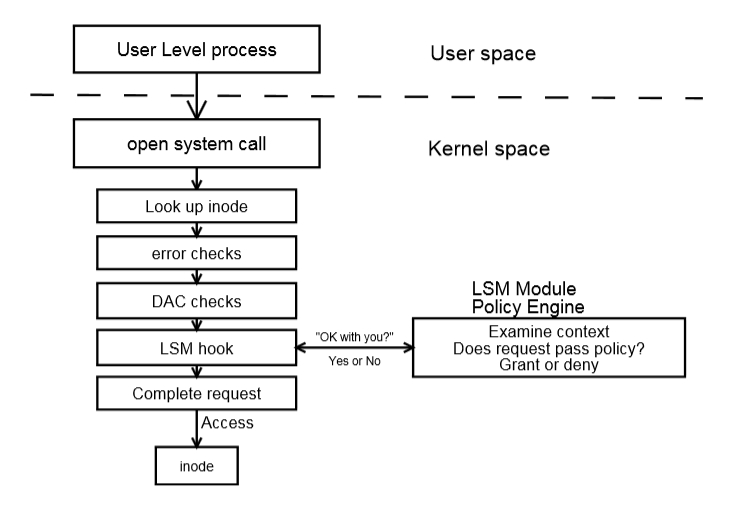
\includegraphics[width=0.9\textwidth]{./images/sec_LSMHook.jpg}
					\caption{Funktionsweise von \emph{System Call}-Hooks eines LSMs \cite[S.3]{LSMFramework}.}
					\label{fig:sec_LSMHook}
			\end{figure}

			Wie in \fig \ref{fig:sec_LSMHook} dargestellt, greift der LSM-Hook erst, wenn ein User einen sicherheitskritischen \emph{System Call} ausführt, die hierbei angefragte Ressource aufgelöst werden, Fehler-Checks abgeschlossen und der Zugriff über den klassischen DAC-Mechanismus genehmigt wurde. Erst wenn der Kernel versucht auf das \glslink{KernelObject}{Kernelobjekt} zuzugreifen, wird der Hook ausgeführt, der den Zugriff in das zugehörige LSM-Modul weiterleitet. Das Modul genehmigt oder verweigert den Zugriff anhand den ihm vorliegenden Zugriffsparametern.

			Der Ausführungszeitpunkt des Hooks bietet den Vorteil, dass der komplette Kontext der Zugriffsanfrage an dieser Stelle vorliegt und vollständig von einem LSM-Modul ausgewertet werden kann \cite[S.2]{LSMFramework}. Zusätzlich wird dadurch die Granularität der Zugriffskontrolle verbessert werden \cite{LSMDesign}.

			% AppArmor und SELinux schuetzen potentiell vor Zero-Day-Exploits.
			%		^		\cite{http://askubuntu.com/questions/485547/contain-docker-engine-with-apparmor}
			% Zero Day Exploit ins Glossar: noch nicht oeffentlich bekannte Sicherheitsluecken in Software

			% Im englischen (linux kernel) "hardening solutions"

			% Siehe \cite[S.5]{dockerSecIntro} rechts unten

			% Zukuenftiger "security namespace", in dnenen jeder Container seine eigenen LSM/MAC dinger definieren kann, je nach sicherheitsanforderung
			%		^ 	\cite[S.17,18]{dockerSec2}

			% S.7 in

			In den folgenden Unterkapiteln werden die beiden MACs \emph{SELinux} und \emph{AppArmor}, sowie deren Einsatzzweck unter Docker vorgestellt. Ein Ausblick in die Zukunft von MACs und Docker ist in Kapitel \ref{result} gegeben.
			% TODO: Checken, ob Referenz wirklich da ist, also Thema in Fazit aufgegriffen ist!

  		\subsubsection{\acrshort{SELinux}}
      	% Macht Sinn das erst am Ende zu machen, wenn noch Zeit ist. Weil SELinux im Detail mehr Exkurs wird.
				\emph{SELinux} steht für \emph{Security Enhanced Linux} und implementiert eine feingranulare MAC, die ursprünglich von der NSA entwickelt wurde. Es wird verwendet, um Anforderungen an die Integrität und Vertraulichkeit von Prozessen und Daten, sowie das \emph{Principle Of Least Privilege} zu realiseren \cite{redhatSec}. %\cite[S.201]{learningDocker}.

				% TODO: Bild aus http://www.admin-magazin.de/Online-Artikel/Mandatory-Access-Control-MAC-mit-SE-Linux hier rein. Bzw. gleiches Bild in \cite[S.63]{linuxMagazineSec}

				Die Beschränkungen beruhen auf einer Sicherheits-Policy, die alle Aktionen zwischen Usern (Subjekten) und Ressourcen (Objekten) regelt. Die Policy besteht aus Anweisungen, die konkrete Sicherheitslabel, wie sie im nächsten Abschnitt beschrieben sind, abbilden. Durch die in \fig \ref{fig:sec_SELinux} dargestellte strikte Trennung des Regelwerks und dessen Durchsetzung, lassen sich mit \emph{SELinux} hohe Sicherheitsanforderungen erfüllen. Durch detailreiche Anpassungsmöglichkeiten steht diese MAC unter dem Ruf besonders schwer konfigurierbar zu sein, obwohl GUI-Tools wie \emph{system-config-selinux} und die Bibliothek \emph{libsemanage} den Umgang mit \emph{SELinux}-Regelwerken in den letzten Jahren vereinfachten \cite[S.62,S.67]{linuxMagazineSec}.
				% cite { https://www.linux.com/learn/docs/727873-overview-of-linux-kernel-security-features/ }
				% cite { https://www.nsa.gov/research/_files/selinux/papers/selsymp2006.pdf }

				Die \emph{Red Hat}-basierten Linux-Distributionen \emph{Red Hat Enterprise Linux}, \emph{Fedora} und \emph{CentOS} sind in der Lage \emph{SELinux} als zusätzlichen Schutzmechanismus zu verwenden \cite{dockerSecurity}.

				\emph{SELinux} kennt das Konzept des DACs von Ownern und Groups nicht. Der komplette Funktionsumfang von \emph{SELinux} beruht auf einem Labeling-System, das Zugriffe individuell für Subjekte verwaltet \cite{SELinuxComic}. In Zuge dessen wird jedem Subjekt zur Laufzeit und jedem Objekt im System ein Label nach dem Schema \texttt{User:Role:Type:Level} zugewiesen \cite{atomicDockerSELinux}. Die erste Komponente \texttt{User} eines Labels ist von einem Linux-Users, der mit \acrshort{DAC} ausgewertet wird, unabhängig.

				\begin{figure}[h]
						\centering
						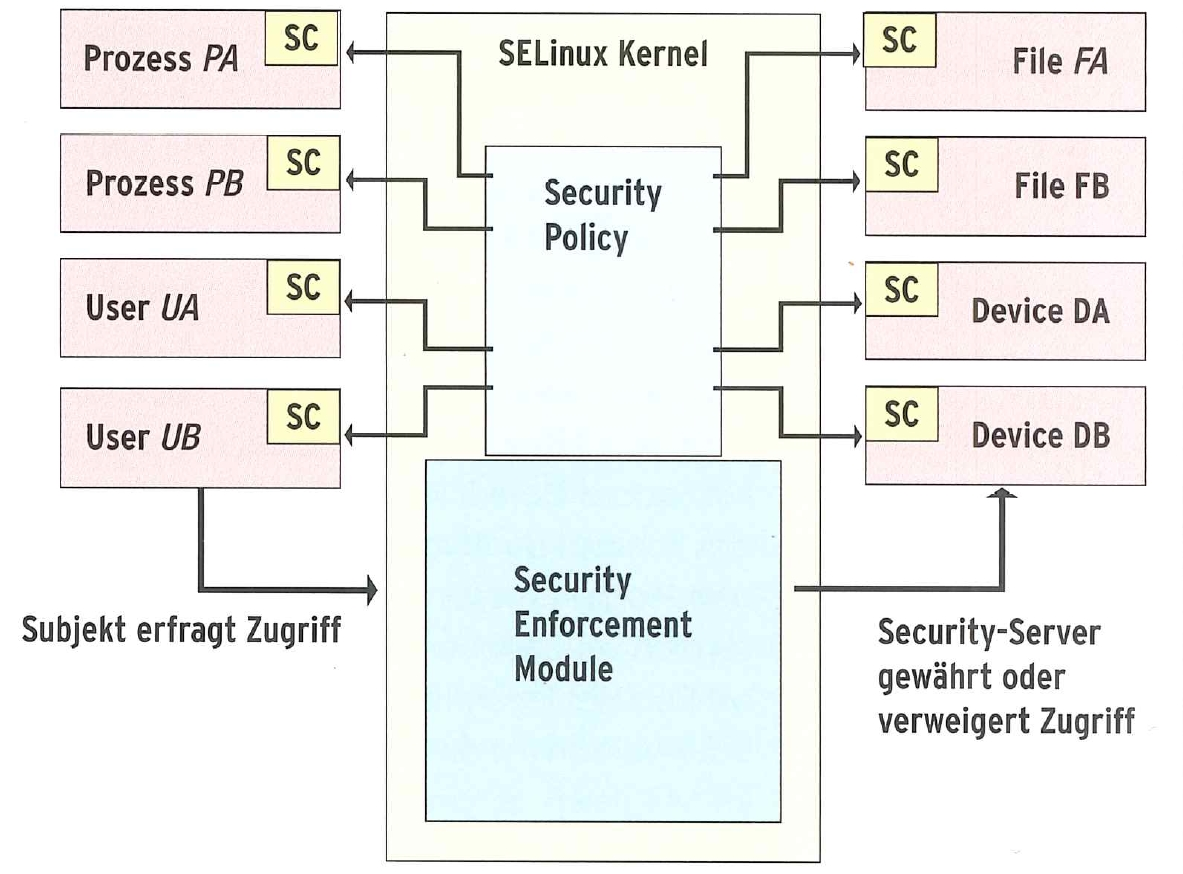
\includegraphics[width=0.9\textwidth]{./images/sec_SELinux.jpg}
						\caption{Trennung von Regelwerk und Enforcement-Modul. Zuweisung von Security-Contexts (SC) an Objekte und Subjekte \cite[S.63]{linuxMagazineSec}.}
						\label{fig:sec_SELinux}
				\end{figure}

				Das Label ist in die erweiternden Attribute (\texttt{xattr}) von Subjekten und Objekts geschrieben \cite[S.65]{linuxMagazineSec}. In \fig \ref{fig:sec_SELinux} ist das Label als \emph{SC} (Security-Context) illustriert.

				% TODO: Label von Prozessen mit Option -Z, also "ps -auxZ", sichtbar
				% Bei Files und Dirs angeblich mit ls --context oder auch -Z moeglich.
				% lstlisting bringen wo die von Docker-Prozessen und /proc /boot files gekennzeichnet sind

				% TODO: SELinux profile unter https://github.com/docker/docker/tree/master/contrib/docker-engine-selinux
				% (ist es wirklich das richtige? das ist in /contrib?) aber evtl auch kompiliert iwo im deb/rpm package mit drin..)
				% |
				% Such a policy is written using a .te file (type enforcement) and an optional .fc file (file contexts) and .if file (interfaces).
				%		^		\cite{https://wiki.gentoo.org/wiki/SELinux/Tutorials/Creating_your_own_policy_module_file}

				\emph{SELinux} wertet bei einem Zugriff das Label des zugreifenden Prozesses und das Label der betroffenen Ressource anhand einem definierten Regelwerk aus und entscheidet, ob die Operation fortgesetzt werden darf \cite{linuxSecOverview}. Die Regeln werden in ihrer Summe auch als Policy bezeichnet.

				Seit November 2015 wird Docker mit dem Release 1.9.0 mit einer standardmäßigen \emph{SELinux}-Policy ausgestattet, die in dem \emph{rpm}-basierten Distributionen wie \emph{CentOS} und \emph{Fedora} verwendet wird \cite{githubDockerChangelog}\cite{githubSELinuxPolicyIssue}. Diese Standard-Policy kann über \cite{githubSELinuxProfile} aufgerufen werden.

				Unter Docker können die vier Label-Attribute mit dem Parameter \texttt{--security-opt="label:LABEL:VALUE"} für den \texttt{run}-Befehl pro Container manuell spezifiziert werden \cite{dockerRun}.

				% TODO: SELinux loggt auch die Zugriffe

				SELinux selbst stellt keine \emph{namespaces} zur Verfügung. Deswegen kann pro Host nur eine SELinux-Policy aktiv sein, die für alle Hostcontainer angewandt wird.

				Auf eine Anwendung abgestimmtes \emph{SELinux}-Regelwerk wird mit der sicherheitskritischen Anwendung zusammen verteilt. Bei der Installation wird dann auch die anwendungsspezifische Policy in das LSM geladen, sodass der Sicherheitsmechanismus nicht manuell eingepflegt werden muss. Außerdem ist die Policy sofort bei der ersten Verwendung der Anwendung aktiv.

				Die \emph{SELinux}-Bausteine, die im Betrieb von Docker eingesetzt werden, sind \emph{Type Enforcement} und \emph{Multi-Category Security} (MCS). Die Eigenheiten beider Mechanismen und deren Funktionsweise unter Docker werden im Folgenden erklärt. Ein weiteres Element \emph{Multi-Level Security} (MLS) wird in dieser Arbeit nicht behandelt, da es unter Docker keine Verwendung findet.
				% Multi-Level Security (MLS) ist verwandt mit MCS. Aber kein Einsatz unter Docker. MLS beruht auf Konzept von "Domination".

				% SELinux funktionert angeblich nicht mit storage driver BRTFS		--> s. auch docker version 1.10 release notes unter security headline
				%		^		\cite{ https://coreos.com/blog/container-security-selinux-coreos.html } --> "notes for deploying"

				% Trennung von Zugriffsdomänen auf zwei Ebenen (TE und MCS)
				%(		^		\cite{learning docker book, see https://books.google.de/books?id=jkkOCgAAQBAJ&pg=PA200&lpg=PA200&dq=mcs+docker&source=bl&ots=0mWUrsFsfO&sig=UXFaVbKKMMXcb_nFW-abQeR0bB0&hl=de&sa=X&ved=0ahUKEwiq5pnLltnKAhUGqA4KHY13AqsQ6AEIXjAI#v=onepage&q=mcs%20docker&f=false .... seite 201}

				% TODO: https://coreos.com/blog/container-security-selinux-coreos.html

				\paragraph{Type Enforcement (TE)}
					Die wichtigste Komponente von \emph{SELinux} ist das \emph{Type Enforcement}. Nach diesem Modell wird jedem Objekt ein Typ zugeweisen, das bei ein Zugriffsoperation ausgewertet wird. Der Typ eines Objekts ist im Label an dritter Stelle definiert.

					Jeder Docker-Prozess hat z.B. im Label den Typ \texttt{docker\_t} definiert. Im \emph{SELinux}-Regelwerk ist festgelegt, dass Prozesse eines Typs nur auf Verzeichnisse und Dateien vollen Zugriff hat, die mit bestimmten Labeltypen versehen sind. Im konkreten Fall von \texttt{docker\_t} umfasst diese Konfiguration ein Set, das z.B. die Typen \texttt{cgroup\_t}, \texttt{docker\_config\_t}, \texttt{docker\_log\_t} und \texttt{svirt\_sandbox\_file\_t} enthält. Versucht ein Docker-Prozess auf Objekte anderer Typen zuzugreifen, wird die Operation unterbunden.

					Da in \emph{SELinux}-Umgebungen jedem Objekt im System ein Label zugewiesen ist, wird eine zuverlässige Kontrolle von Objektzugriffen über die Auswertung von Typen ermöglicht. Prozesse, die mit dem Typ \texttt{docker\_t} aus der Docker-Domäne stammen, sind streng von Objekten anderer Domänen abgegrenzt und können nicht interagieren.
					% We label Apache processes as httpd_t and we label Apache content as httpd_sys_content_t and httpd_sys_content_rw_t. Imagine we have credit card data stored in a mySQL database which is labeled msyqld_data_t. If an Apache process is hacked, the hacker could get control of the httpd_t process and would be allowed to read httpd_sys_content_t files and write to httpd_sys_content_rw_t. But the hacker would not be allowed to read the credit card data (mysqld_data_t) even if the process was running as root. In this case SELinux has mitigated the break in.
					% Standardmäßig ist ein Zugriff verweigert. Erst wenn Labels uebereinstimmen, wird Zugriff erlaubt.
					% 	^		\cite{SELinuxComic}

					% Type enforcement is a kind of enforcement in which rules are based on process type. It works in the following way. The default type for a confined container process is svirt_lxc_net_t. This type is permitted to read and execute all files "types" under /usr and most types under /etc. svirt_lxc_net_t is permitted to use the network but is not permitted to read content under /var, /home, /root, /mnt … svirt_lxc_net_t is permitted to write only to files labeled svirt_sandbox_file_t and docker_var_lib_t. All files in a container are labeled by default as svirt_sandbox_file_t. Access to docker_var_lib_t is permitted in order to allow the use of docker volumes \cite{ http://www.projectatomic.io/docs/docker-and-selinux/ }.

				\paragraph{Multi-Category Security (MCS)}
					% TODO: Einarbeiten, dass mit Kateogiren die Vertraulichkeit erfüllt wird: Kategorisierung führt dazu, dass nur solche Prozesse auf Objekte haben, die derselben Kategorie angehören.
					% TODO: Systemintegrität und Domänen mit Type Enforcement realisiert! Prozesse laufen innerhalb einer Domäne und Objekte haben einen Typ. Durch Regeln wird bestimmt, welche Domänen auf welche Typen zugreifen dürfen.
					Durch das einheitliche Regelwerk für alle Docker-Prozesse, ist mit einem \emph{Type Enforcement} gewährleistet, dass Docker nicht unbefugt auf geschützte oder unrelevante Dateien des Hosts zugreifen darf.

					\emph{SELinux} bietet mit dem MCS-Mechanismus jedoch auch eine Möglichkeit, Docker-Prozesse untereinander zu trennen, auch wenn sie den gleichen Typ, z.B. \texttt{docker\_t} aufweisen. Dieses Sicherheitsfeature ist unter Docker auch mit \emph{Type Enforcements} realisierbar, wenn jeder Container mit einem eigenen Typ operiert. Diese feinere Typenunterteilung wirkt sich aber auf die Komplexität der Policy aus, weswegen in der Regel der MCS-Mechanismus für dieses Sicherheitsfeature eingesetzt wird.
					% TODO: Quelle!
					% ist aber sehr aufwendig...
					% \cite{https://securityblog.redhat.com/tag/docker/}

					Der MCS-Mechanismus arbeitet mit dem letzten Teil des Labels, dem \texttt{Level}. Das Level unterteilt sich mit der Schreibweise \texttt{sensitivity[:category-set]} in eine Sensitivität, oder auch Schutzstufe genannt, und optionalen Kategorien. Für die MCS sind die Kategorien von Bedeutung. Die Schutzstufe wird ignoriert, weil sie nur unter der nicht von Docker verwendeten \acrshort{MLS} Anwendung findet. Im Fall von Docker hat die Schutzstufe deswegen einen konstanten Wert von \texttt{s0}.
					% TODO: Quellen!
					%\cite{ https://access.redhat.com/documentation/en-US/Red_Hat_Enterprise_Linux/6/html/Security-Enhanced_Linux/chap-Security-Enhanced_Linux-SELinux_Contexts.html } \cite{ http://james-morris.livejournal.com/5583.html }

					Beim Startvorgang eines Containers wird diesem eine zufällige Kategorie anhand einer Nummer zwischen 0 und 1023 zugeweisen. Diese Kategorie, z.B. \texttt{c623}, wird daraufhin auch vom Docker-Daemon auf den Inhalt containerspezifischer Verzeichnisse angewandt. Sobald während des Betriebs ein Container Zugriff auf ein Objekt fordert, wird seine Kategorie mit dem des angefragten Objekts verglichen. Stimmen diese überein, ist der MCS-Check erfolgreich und der Zugriff wird freigegeben.
					% Quelle!
					% \cite{learningDocker}.

					Die Sicherheit von MCS unter Docker beruht auf der Annahme, dass der Docker-Daemon zuverlässig eindeutige Kategorien an die Container vergibt.
					% Quelle!
					% war glaub ich auch aus learningDocker....s201

					Falls ein Angreifer einen Container unter Kontrolle hat, ist es ihm durch die MCS nicht möglich, außerhalb von dem komprmitiertem Container Schaden anzurichten.
					% Verständnisproblem: Auch wenn Angreifer Root-Rechte erwirkt? Ist er dann noch "im Container"?


					% n computer systems we often have lots of processes all with the same access, but we want them separated from each other. We sometimes call this a multi-tenant environment. The best example of this is virtual machines. If I have a server running lots of virtual machines, and one of them gets hacked, I want to prevent it from attacking the other virtual machines and virtual machine images. But in a type enforcement system the KVM virtual machine is labeled svirt_t and the image is labeled svirt_image_t. We have rules that say svirt_t can read/write/delete content labeled svirt_image_t. With libvirt we implemented not only type enforcement separation, but also MCS separation. When libvirt is about to launch a virtual machine it picks out a random MCS label like s0:c1,c2, it then assigns the svirt_image_t:s0:c1,c2 label to all of the content that the virtual machine is going to need to manage. Finally, it launches the virtual machine as svirt_t:s0:c1,c2. Then, the SELinux kernel controls that svirt_t:s0:c1,c2 can not write to svirt_image_t:s0:c3,c4, even if the virtual machine is controled by a hacker and takes it over. Even if it is running as root.

					% We use similar separation in OpenShift. Each gear (user/app process)runs with the same SELinux type (openshift_t). Policy defines the rules controlling the access of the gear type and a unique MCS label to make sure one gear can not interact with other gears.

				\paragraph{Multi-Level Security (MLS)}
					\emph{DELETE -- MLS nicht unter Docker genutzt...}
					% Arbeitet MLS nur auf s0...sX ebene und ignoriert c0..cX?

					% MLS enforces the Bell-La Padula Mandatory Access Model
					%		^		\cite{ https://access.redhat.com/documentation/en-US/Red_Hat_Enterprise_Linux/6/html/Security-Enhanced_Linux/chap-Security-Enhanced_Linux-SELinux_Contexts.html }

					% I could have two Apache servers: one running as httpd_t:TopSecret and another running as httpd_t:Secret. If the Apache process httpd_t:Secret were hacked, the hacker could read httpd_sys_content_t:Secret but would be prevented from reading httpd_sys_content_t:TopSecret.

					% However, if the Apache server running httpd_t:TopSecret was hacked, it could read httpd_sys_content_t:Secret data as well as httpd_sys_content_t:TopSecret.

					% We use the MLS in military environments where a user might only be allowed to see secret data, but another user on the same system could read top secret data.

					%------

					% The Multi-Level Security technology refers to a security scheme that enforces the Bell-La Padula Mandatory Access Model. Under MLS, users and processes are called subjects, and files, devices, and other passive components of the system are called objects. Both subjects and objects are labeled with a security level, which entails a subject's clearance or an object's classification. Each security level is composed of a sensitivity and a category, for example, an internal release schedule is filed under the internal documents category with a confidential sensitivity.

      \subsubsection{AppArmor}
      	% Optional, da auf MAC alzu sehr eingehen nicht zu sehr im Scope sein sollte.
				AppArmor implementiert als LSM auch eine MAC, wurde jedoch als leicht konfigurierbare Alternative zu \emph{SELinux} entwickelt. Es kommt in Linuxdistributionen wie \emph{Debian}, \emph{Ubuntu} und \emph{OpenSUSE} standardmäßig zum Einsatz \cite{apparmorUbuntu}.
				% Einfach zu lernen
				% Basiert auf \emph{AppArmor}-Profilen.
				% Es gibt von \emph{Docker} erstelltes Profil, das speziell für den Einsatz von Docker mit \emph{AppArmor} gebaut wurde. \cite{ https://docs.docker.com/engine/articles/security/ }



				Der fundamentale Unterschied zu \emph{SELinux} ist, dass Objekten keine Label zugeweisen werden, sondern grundsätzlich Pfadnamen und sieben Berechtigungstypen dazu dienen, ein Sicherheitsprofil zu definieren \cite{linuxSecOverview}\cite{apparmorQuickProfileLanguage}.

				% AppArmor profiles can be in one of two modes: enforcement and complain. Profiles loaded in enforcement mode will result in enforcement of the policy defined in the profile as well as reporting policy violation attempts (either via syslog or auditd). Profiles in complain mode will not enforce policy but instead report policy violation attempts.
				% AppArmor differs from some other MAC systems on Linux: it is path-based, it allows mixing of enforcement and complain mode profiles, it uses include files to ease development, and it has a far lower barrier to entry than other popular MAC systems.
				%		^		\cite{ https://wiki.ubuntu.com/AppArmor }

				\emph{AppArmor} unterstützt einen Lernmodus, indem das Verhalten einer Anwendungen beobachtet wird und daraus automatisch ein Sicherheitsprofil erstellt wird \cite{linuxSecOverview}.
				% TODO: Complain mode, enforce mode etc. weiter ausfuehren. --> Liste der 3? verschiednen modi
				% enforce modus:  actively block and audit in dmesg anything outside the bounds of the docker-default profile. \cite{githubAppArmorDoc}
				% und "sudo aa-status" beweist, dass docker-default im enforce-mode laeuft.

				\emph{AppArmor}-Profile basieren auf einfach lesbaren Textdateien. Durch eine Inkludieranweisung lassen sich mehrere Profile modular kombinieren \cite{apparmorQuickProfileLanguage}.
				% Capabilities und Networking lassen sich beide kontrollieren mit AppArmor

				Das Standardprofil \texttt{docker-default} \cite{githubAppArmorProfileContainer}, das im \texttt{enforce}-Modus unter \emph{.deb}-Releases in nicht-priveligierten Containern zum Einsatz kommt \cite{docker110Security}, wird bei der Installation von Docker in die Datei \texttt{/etc/apparmor.d/docker} geschrieben. Administratoren können sich mit dem Befehl \texttt{sudo aa-status} vergewissern, ob das Standardprofil aktuell aktiv ist. Auch die zurückgegebenen Sicherheitskontexte in der ersten Spalte von \fig ... und \fig ... belegen die standardmäßige Verwendung von \texttt{docker-default}.

				Das \emph{AppArmor}-Profil kann mit dem \texttt{run}-Parameter \texttt{--security-opt="apparmor:PROFILE"} manuell überschrieben werden, sofern dieses in \emph{AppArmor}, z.B. mit dem \acrshort{CLI}-Tool \texttt{apparmor\_parser} \cite{apparmorParser}, zuvor importiert wurde \cite{dockerRun}.

				Das Profil \texttt{docker-default} wurde erst kürzlich während der Erstellung dieser Arbeit aktualisiert. Aus der Commit-Nachricht geht allerdings nicht hervor, ob damit eine Sicherheitslücke geschlossen wurde oder die Änderungen im Zuge einer Funktionsänderung von Containern entstanden sind \cite{githubAppArmorProfileContainerFix}. Die aktuelle Implementierung des Profils, die mit dem Konsolenbefehl \texttt{cat /etc/apparmor.d/docker} ausgegeben werden kann, sieht folgende \emph{AppArmor}-Regeln vor:

				\begin{lstlisting}
					#include <tunables/global>

					profile docker-default flags=(attach_disconnected,mediate_deleted) {
					  #include <abstractions/base>

					  network,
					  capability,
					  file,
					  umount,

					  deny @{PROC}/{*,**^[0-9*],sys/kernel/shm*} wkx,

						deny @{PROC}/* w,
						deny @{PROC}/{[^1-9],[^1-9][^0-9],[^1-9s][^0-9y][^0-9s],[^1-9][^0-9][^0-9][^0-9]*}/** w,
						deny @{PROC}/sys/[^k]** w,
						deny @{PROC}/sys/kernel/{?,??,[^s][^h][^m]**} w,

					  deny @{PROC}/sysrq-trigger rwklx,
					  deny @{PROC}/mem rwklx,
					  deny @{PROC}/kmem rwklx,
					  deny @{PROC}/kcore rwklx,

					  deny mount,

					  deny /sys/[^f]*/** wklx,
					  deny /sys/f[^s]*/** wklx,
					  deny /sys/fs/[^c]*/** wklx,
					  deny /sys/fs/c[^g]*/** wklx,
					  deny /sys/fs/cg[^r]*/** wklx,
					  deny /sys/firmware/efi/efivars/** rwklx,
					  deny /sys/kernel/security/** rwklx,
					}
				\end{lstlisting}
				\emph{Evtl. in Anhang damit}
				% TODO: Erklaerungen teilweise in https://github.com/docker/docker/commit/2b4f64e59018c21aacbf311d5c774dd5521b5352
				% TODO: Inhalt der Datei in den Anhang oder als Codeblock an diese Stelle? 1. cat /etc/apparmor.d/docker ..... 2. \cite{githubAppArmorDoc}
				% TODO: abstractions sind erklaert in https://books.google.de/books?id=1hVmn4RnKH0C&pg=PA97&lpg=PA97&dq=apparmor+abstractions+base&source=bl&ots=O7scPJ76X8&sig=FNYnyDrkfj3T-uOL1CGZbpcc_5s&hl=de&sa=X&ved=0ahUKEwjU9NPn5OrKAhWEFSwKHZAsDOYQ6AEIYDAI#v=onepage&q=apparmor%20abstractions%20base&f=false

				Es existiert auch ein Profil für den Docker-Daemon \cite{githubAppArmorProfileDaemon}, allerdings muss dieses manuell aktiviert werden \cite{githubAppArmorDoc}.

    \subsection{Seccomp}
			% TODO: https://lwn.net/Articles/443099/ und https://lwn.net/Articles/441232/
			% TODO: und vllt https://lwn.net/Articles/443110/

			\emph{Seccomp} steht für \emph{Secure Computing Mode} und setzt einen von \emph{Google} implementierten Mechanismus um, der den Zugriff von Prozessen auf \emph{System Calls} einschränkt. Die Idee von \emph{Seccomp} ist es, die Angriffsfläche des Kernels zu minimieren, indem bestimmte \emph{System Calls} für Useranwendungen gesperrt werden. Die Gefahr, dass fehlerbehaftete oder unsichere \emph{System Calls} genutzt werden, die die Anwendung zum fehlerfreien Betrieb nicht benötigt, wird dadurch reduziert \cite{linuxSecOverview}\cite{seccompGitDesc}\cite{secInFuture}.

			\emph{Seccomp} ist nicht wie \emph{SELinux} und \emph{AppArmor} als LSM implementiert, sondern arbeitet auf Applikationslevel.
			% \emph{SO NICHT RICHTIG, siehe https://github.com/docker/docker/blob/master/docs/security/seccomp.md}.
			%	Secure computing mode (Seccomp) is a Linux kernel feature. You can use it to restrict the actions available within the container. The seccomp() system call operates on the seccomp state of the calling process. You can use this feature to restrict your application's access.
			% This feature is available only if the kernel is configured with CONFIG_SECCOMP enabled.

			Das hat die positive Auswirkung, dass \emph{Seccomp}-Profile auch von nicht-priveligierten Nutzern geladen werden können. Mit LSMs ist dies nicht möglich.
			% 	^		\cite{ https://lwn.net/Articles/443099/ }
			Die Verwendung von \emph{Seccomp} für einen Prozess bewirkt, dass jener in einen \glqq{}sicheren\grqq{} Zustand übergeht, sodass er nur noch fest definierte \emph{System Calls} ausführen kann.
			%		^		\cite{ wikipedia :( }

			% x86_x64 hat mehr als 600 System Calls. bzw. mehrere hundert
			%		^		\cite{ https://opensource.com/business/15/3/docker-security-future }

			% This feature is available only if the kernel is configured with CONFIG_SECCOMP enabled.
			%		^		\cite{ https://github.com/docker/docker/blob/master/docs/security/seccomp.md }

			Das originale Seccomp, auch als \emph{mode 1} bekannt, stellt nur den Zugriff auf vier \emph{System Calls} zur Verfügung: \texttt{read}, \texttt{write}, \texttt{exit} und \texttt{sigreturn}. Diese vier Aufrufe repräsentieren ein minimales Set an Operationen, die eine nicht vertrauenswürdige Anwendung ausführen darf \cite{linuxSecOverview}.

			Ein Update \emph{mode 2} macht das Set an erlaubten \emph{System Calls} mithilfe von Filtern frei konfigurierbar und führt ein \emph{Audit Logging} ein	\cite{linuxSecOverview}\cite{seccompGitDesc}.

			Mithilfe der \emph{Seccompn}-Anweisungen \texttt{allow}, \texttt{deny}, \texttt{trap}, \texttt{kill} und \texttt{trace} sind neben der Sperrung noch weitere Aktionen, die zur Kontrolle von \emph{System Calls} dienen, möglich \cite{docker110Security}.

			Seit Oktober 2015 ist eine \emph{Seccomp}-Unterstützung in Planung und Entwicklung \cite{githubGeneralSecProfiles}\cite{githubSeccompIntegration}. Diese wurde in Form eines \emph{Seccomp}-Standardprofils sowie der Option eigene Profile einzubinden, der zum Erstellungszeitpunkt dieser Arbeit neusten Docker-Version 1.10 am 04. Februar 2016 hinzugefügt \cite{githubDockerChangelog}\cite{githubSeccompDoc}
			\cite{githubSeccompProfile}\cite{docker110Security}. Das Standardprofil basiert seit Ende 2015 auf einer Whitelist (davor einer Blacklist), sprich es blockiert, abgesehen von den in dieser Liste aufgeführten Operationen, alle \emph{System Calls} \cite{githubSeccompDoc}.

			Eine aktuelle Liste der explizit erlaubten und resultierend blockierten Aufrufe ist in \cite{githubSeccompProfile} und \cite{githubSeccompDoc} zu finden.

			Seit der Umstellung von Blacklisting auf Whitelisting wurde die \emph{System Call}-Auflistung in einem Zeitraum von ca. fünf Wochen 47 Änderungen unterzogen. Davon sind 40 Neueinträge und sieben Löschungen zu registrieren \cite{githubSeccompProfileHistory}. Während sich es bei den Neueinträgen um bewusste Funktionserweiterungen handeln kann, werfen sieben Löschungen den Verdacht auf, dass das \emph{Seccomp}-Standardprofil weder als vollständig noch ausreichend getestet betrachtet werden kann.
			% TODO: CHECK AGAIN nach commit history aenderungen!

			Die offizielle Dokumentation des \texttt{run}-Befehls sieht noch keine Anpassungsmöglichkeit von \emph{Seccomp} vor \cite{dockerRun}. Jedoch ist an anderer Stelle im \emph{GitHub}-Repository vermerkt, dass sich das Standardprofil mit dem Parameter \texttt{--security-opt seccomp:PROFILEPATH} überschreiben lässt \cite{githubSeccompDoc}. Ist es nötig, Container ohne \emph{Seccomp} zu starten, kann das mit der Option \texttt{--security-opt seccomp:unconfined} realisiert werden \cite{docker110Security}.

	\section{Docker im Vergleich zu anderen Containerlösungen}
  	% Optional?

		% Vergleich von CoreOs 1.0 und Docker 1.10?

		% Selbst steinaltes OpenBSD baut noch an tame() / neu:pledge() -Funktion rum, um soetwas wie Seccomp zu ermoeglichen
		%	Tame() als Vorbild fuer general framework von docker (siehe RFC github post von frazelli) --> Mehr in Fazit-Kapitel rein.
		%		^		\cite{https://news.ycombinator.com/item?id=10537268}

		% Von CoreOS-Website: Security-minded capabilities
		% rkt is built from the ground up to be ready for security-focused environments. Many of these principles weren’t invented at CoreOS — instead, we applied common, everyday best practices that have been largely overlooked in the container industry so far.

\end{document}
